\documentclass{article}
\usepackage{graphicx}
\usepackage{amsthm}
\usepackage{amsmath}
\usepackage{amssymb}
\usepackage{geometry}
\usepackage{tikz}
\usetikzlibrary{arrows}

\geometry{a4paper, total={170mm,257mm}, left=20mm, top=20mm}
\AtBeginEnvironment{align}{\setcounter{equation}{0}} 
\AtBeginEnvironment{eqnarray}{\setcounter{equation}{0}} 

\title{HW9 (CSCI-C241)}
\author{Lillie Donato}
\date{26 March 2024}

\begin{document}

\maketitle

\begin{enumerate}
    \item Question One
    \begin{enumerate}
        \item $\forall x ((A(x) \lor B(x)) \rightarrow (C(x) \land \neg D(x)))$
        \item $\neg \exists x (A(x) \land B(x))$
    \end{enumerate}
    \item Question Two
    \begin{enumerate}
        \item $\mathcal{U}_1, \mathcal{U}_2, \mathcal{U}_5, \mathcal{U}_6, \mathcal{U}_7$
        \item $\mathcal{U}_1, \mathcal{U}_6, \mathcal{U}_7, \mathcal{U}_8$
        \item $\mathcal{U}_7$
        \item $\mathcal{U}_3, \mathcal{U}_4, \mathcal{U}_8$
        \item $\mathcal{U}_2, \mathcal{U}_3, \mathcal{U}_4, \mathcal{U}_5$
        \item $\mathcal{U}_2, \mathcal{U}_3, \mathcal{U}_4, \mathcal{U}_5$
        \item $\mathcal{U}_3, \mathcal{U}_4, \mathcal{U}_8$
        \item Part (h)
        \begin{enumerate}
            \item $\neg \forall x (L(x) \rightarrow V(x))$ and $\exists x (L(x) \land \neg V(x))$
            \item $\forall x (L(x) \rightarrow \neg V(x))$ and $\neg \exists x (L(x) \land V(x))$
        \end{enumerate}
    \end{enumerate}
    \item Question Three
    \begin{enumerate}
        \item 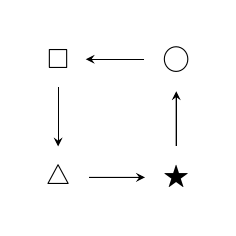
\begin{tikzpicture}[scale=1.5, node distance={15mm}, main/.style = {circle}]
            % Nodes
            \node[main] (1) {$\square$};
            \node[main] (2) [below of=1] {$\triangle$};
            \node[main] (3) [right of=1] {$\bigcirc$};
            \node[main] (4) [below of=3] {$\bigstar$};

            % Loops
            % \draw[->,>=stealth] (1) edge[out=120, in=60, looseness=5] (1);
            
            % Lines
            \draw[->, >=stealth] (1) -- (2);
            \draw[->, >=stealth] (2) -- (4);
            \draw[->, >=stealth] (4) -- (3);
            \draw[->, >=stealth] (3) -- (1);
        \end{tikzpicture}
        \item 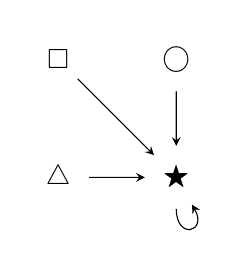
\begin{tikzpicture}[scale=1.5, node distance={15mm}, main/.style = {circle}]
            % Nodes
            \node[main] (1) {$\square$};
            \node[main] (2) [below of=1] {$\triangle$};
            \node[main] (3) [right of=1] {$\bigcirc$};
            \node[main] (4) [below of=3] {$\bigstar$};

            % Loops
            \draw[->,>=stealth] (4) edge[out=270, in=300, looseness=5] (4);
            
            % Lines
            \draw[->, >=stealth] (1) -- (4);
            \draw[->, >=stealth] (2) -- (4);
            \draw[->, >=stealth] (3) -- (4);
        \end{tikzpicture}
        % \item This is not possible as, $\exists y \forall x P(x, y)$ states that there exists a shape $x$ such that every shape points to, but on the other hand $\forall x \exists y P(x,y)$ which must be false, states that for every shape, there exists a shape $y$ such that the first shape points to, meaning not every shape can point to another. With that being said, if not every shape can point to another, then a shape that has every shape pointing to itself can't exist.
        \item $\mathcal{M}_1, \mathcal{M}_2, \mathcal{M}_3$
        \item $\mathcal{M}_2$
        \item $\mathcal{M}_{10}$
    \end{enumerate}
    \item Question Four
    \begin{enumerate}
        \item $\forall x \forall y \forall z (\exists w R(x, w) \land ((R(x,y) \land R(x,z)) \rightarrow y = z))$
    \end{enumerate}
    \item Question Five
    \begin{enumerate}
        \item $\forall x (A(x) \rightarrow ((\exists y (B(y) \land R(x,y))) \land (\forall y \forall z ((B(y) \land B(z)) \rightarrow ((R(x,y) \land R(x,z)) \rightarrow y = z)))))$
    \end{enumerate}
    \item Question Six
    \begin{enumerate}
        \item $5! = 1 \cdot 2 \cdot 3 \cdot 4 \cdot 5 = 120$
        \item $n-1$
        \item $n+1$
        \item $n$
        \item $(k+1) \cdot k!$
    \end{enumerate}
    \item Question Seven
    \begin{enumerate}
        \item Claim: $n \geq 2$, $3^n > 2^{n+1}$
        \begin{proof}
            (induction on $n$) \\
            (Base Step, $n=2$):
            \begin{eqnarray}
                3^2 &=& 9 \\
                &>& 8 \\
                &=& 2^3 \\
                &=& 2^{2+1}
            \end{eqnarray}
            (Inductive Step): \\
            Assume $3^k > 2^{k+1}$ for some $k \geq 2$ \\
            \begin{eqnarray}
                3^{k+1} &=& 3^k \cdot 3^1 \\
                &=& 3^k \cdot 3 \\
                &>& 2^{k+1} \cdot 2 \hspace{1cm} \text{(by the induction hypothesis, and $3 > 2$)}\\
                &=& 2^{k+1+1}
            \end{eqnarray}
        \end{proof}
        \item Claim: $n \geq 9$, $3^n < (n-1)!$
        \begin{proof}
            (induction on $n$) \\
            (Base Step, $n=9$):
            \begin{eqnarray}
                3^9 &=& 19683 \\
                &<& 40320 \\
                &=& 8! \\
                &=& (9-1)!
            \end{eqnarray}
            (Inductive Step): \\
            Assume $3^k < (k-1)!$ for some $k \geq 9$
            \begin{eqnarray}
                3^{k+1} &=& 3^k \cdot 3 \\
                &<& (k-1)! \cdot k \hspace{1cm} \text{(by the induction hypothesis, and $k > 3$)}\\
                &=& k! \\
                &=& (k-1+1)!
            \end{eqnarray}
        \end{proof}
        \item Claim: $n \geq 2$, $3^n > n^2$
        \begin{proof}
            (induction on $n$) \\
            (Base Step, $n=2$):
            \begin{eqnarray}
                3^2 &=& 9 \\
                &>& 4 \\
                &=& 2^2
            \end{eqnarray}
            (Inductive Step): \\
            Assume $3^k > k^2$ for some $k \geq 2$
            \begin{eqnarray}
                3^{k+1} &=& 3^k \cdot 3 \\
                &>& k^2 \cdot 3 \hspace{1cm} \text{(by the induction hypothesis)} \\
                &=& k^2 + k^2 + k^2 \\
                &\geq& k^2 + 2k + 1 \hspace{1cm} \text{($k^2 \geq 2k > 1$ for all $k \geq 2$)}\\
                &=& (k+1)(k+1) \\
                &=& (k+1)^2
            \end{eqnarray}
        \end{proof}
        \item Claim: $n^2 -3n$ is even for all $n \in \mathbb{N}$
        \begin{proof}
            (induction on $n$) \\
            (Base Step, $n = 0$):
            \begin{eqnarray}
                0^2 - 3(0) &=& 0 - 0 \\
                &=& 0
            \end{eqnarray}
            \hspace{1cm} $0$ is even

            (Inductive Step): 

            \hspace{1cm} Assume $k^2 -3k$ is even for all $k \in \mathbb{N}$ 

            \hspace{1cm} $k^2-3k = 2c_1$
            \begin{eqnarray}
                (k+1)^2 - 3(k+1) &=& (k+1)(k+1) -3k -3 \\
                &=& k^2 + 2k + 1 - 3k - 3 \\
                &=& (k^2 - 3k) + (2k - 2) \\
                &=& (k^2 - 3k) + 2(k-1) \\
                &=& 2c_1 + 2(k-1) \hspace{1cm} \text{(by the induction hypothesis)} \\
                &=& 2c_1 + 2c_2 \hspace{1cm} \text{(Let $c_2 = k-1$)} \\
                &=& 2(c_1 + c_2) \\
                &=& 2c_3 \hspace{1cm} \text{(Let $c_3 = c_1 + c_2$)} \\
                &&2c_3 \text{ is even} \hspace{1cm} \text{($2n$ is even, where $n \in \mathbb{N}$)} \\
            \end{eqnarray}
            \hspace{1cm} Since $2c_3$ is even, $(k+1)^2 - 3(k+1)$ is even
        \end{proof}
        \item Claim: There are $2^n$ binary string of length $n$ for all $n \in \mathbb{N}$
        \begin{proof}
            (induction on $n$) \\
            (Base Step, $n=0$):
            \begin{eqnarray}
                2^0 &=& 1
            \end{eqnarray}
            \hspace{1cm} There is only one possible binary string, of length $0$, the empty string.

            (Inductive Step):

            \hspace{1cm} Assume for length $k$, there are $2^k$ binary strings
            \begin{eqnarray}
                &&\text{For every binary string of length $k$, there are $2^k$ binary strings,} \\
                &&\hspace{1cm} \text{for each binary string, there are two new possible binary strings of length $k+1$,} \\
                &&\text{So, by the induction hypothesis there are $2^k \cdot 2$ binary strings of length $k+1$}
            \end{eqnarray}
        \end{proof}
        \item Claim: For any set of characters, with the length of $a$ and any $n \in \mathbb{N}$, there are $a^n$ possible strings of length $n$ that explicitly use the said alphabet
        \begin{proof}
            (induction on $n$) \\
            (Base Step, $n=0$):
            \begin{eqnarray}
                a^0 &=& 1
            \end{eqnarray}
            \hspace{1cm} Regardles of the possible characters, there is only one possible string, of length $0$, the empty string.

            (Inductive Step):

            \hspace{1cm} Assume for length $k$, there are $a^k$ strings, where $a$ is total amount of different characters
            \begin{eqnarray}
                && \text{For every string of length $k$, there are $a$ possible different characters,} \\
                && \hspace{1cm} \text{and $a^k$ possible strings} \\
                && \text{For every string of length $k+1$, with the same $a$ possible characters,} \\
                && \hspace{1cm} \text{for each string, there would $a$ possible new strings of length $k+1$} \\
                &&\text{So, by the induction hypothesis there are $a^k \cdot a$ strings of length $k+1$}
            \end{eqnarray}
        \end{proof}
    \end{enumerate}
\end{enumerate}

\end{document}